%\documentclass[mathserif]{beamer}
\documentclass[handout]{beamer}
%\usetheme{Goettingen}
\usetheme{Warsaw}
%\usetheme{Singapore}
%\usetheme{Frankfurt}
%\usetheme{Copenhagen}
%\usetheme{Szeged}
%\usetheme{Montpellier}
%\usetheme{CambridgeUS}
%\usecolortheme{}
%\setbeamercovered{transparent}
\usepackage[english, activeacute]{babel}
\usepackage[utf8]{inputenc}
\usepackage{amsmath, amssymb}
\usepackage{dsfont}
\usepackage{graphics}
\usepackage{cases}
\usepackage{graphicx}
\usepackage{pgf}
\usepackage{epsfig}
\usepackage{amssymb}
\usepackage{multirow}	
\usepackage{amstext}
\usepackage[ruled,vlined,lined]{algorithm2e}
\usepackage{amsmath}
\usepackage{epic}
\usepackage{epsfig}
\usepackage{fontenc}
\usepackage{framed,color}
\usepackage{palatino, url, multicol}
\usepackage{listings}
%\algsetup{indent=2em}
\vspace{-0.5cm}
\title{Descriptive Statistics}
\vspace{-0.5cm}
\author[Felipe Bravo Márquez]{\footnotesize
%\author{\footnotesize  
 \textcolor[rgb]{0.00,0.00,1.00}{Felipe José Bravo Márquez}} 
\date{ \today }


\begin{document}
\begin{frame}
\titlepage


\end{frame}


%%%%%%%%%%%%%%%%%%%%%%%%%%%






\begin{frame}{Exploratory Data Analysis}
\scriptsize{
\begin{itemize}
 \item Descriptive Statistics or Exploratory Data Analysis or (EDA) encompasses a set of techniques to quickly understand the nature of a data collection or \textbf{dataset}.
 
 \item The main goal of descriptive statistics is to explore the data to find some patterns that can be exploited to generate hypotheses.
 
 \item It was proposed by the statistician John Tukey.
 
 \item It is based mainly on two types of techniques: \textbf{summary statistics} and \textbf{data visualization}.
 
 \item In this class you will see both types of techniques, in addition to their application in R for some toy datasets.
 
 \item This class in partially based on chapter 3 of \cite{tan2016introduction}.  
 
\end{itemize}

}

\end{frame}

\begin{frame}{The Iris dataset}
\scriptsize{
\begin{itemize}
 \item We will work with a well-known dataset called \textbf{Iris}.
 \item The dataset consists of 150 observations of iris plant flowers. 
 \item There are three types of iris flower classes: \textbf{virginica}, \textbf{setosa} and \textbf{versicolor}.
 \item There are 50 observations of each.
\item The variables or attributes measured for each flower are:

\begin{enumerate}
\scriptsize{
  \item The type of flower as a categorical variable.
 \item The length and width of the petal in cm as numerical variables.
 \item The length and width of the sepal in cm as numeric variables.
  }
\end{enumerate}

 
\end{itemize}


\begin{figure}[h!]
	\centering
	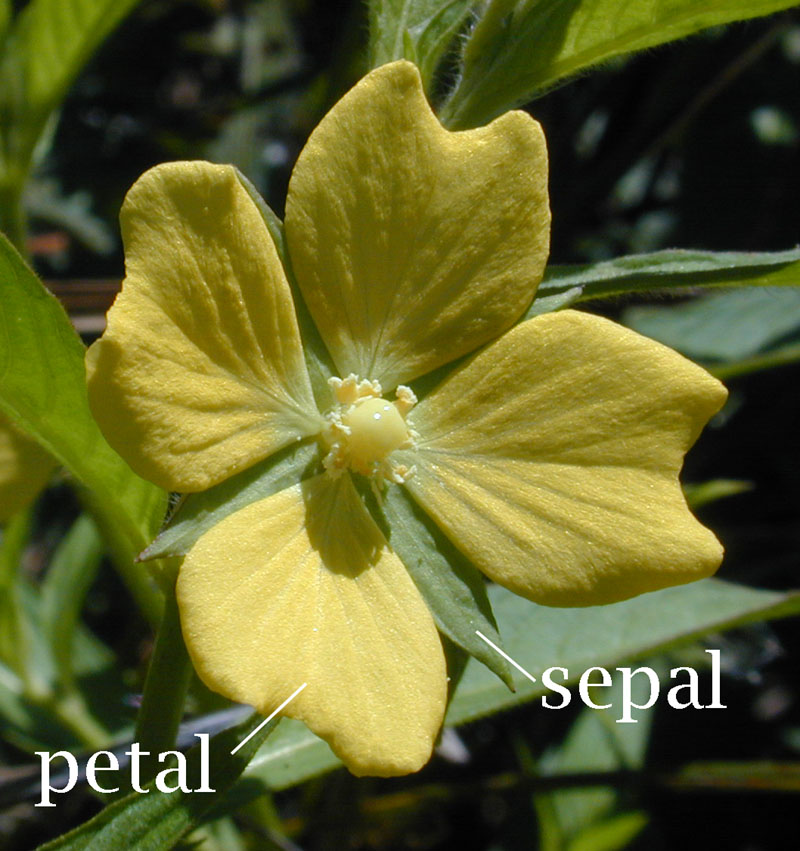
\includegraphics[scale=0.4]{pics/Petal-sepal.jpg}
	
	
\end{figure}

}

\end{frame}

\begin{frame}[fragile]{The Iris dataset}
\scriptsize{


 \begin{figure}[h!]
\begin{center}
\begin{tabular}{ccc}
 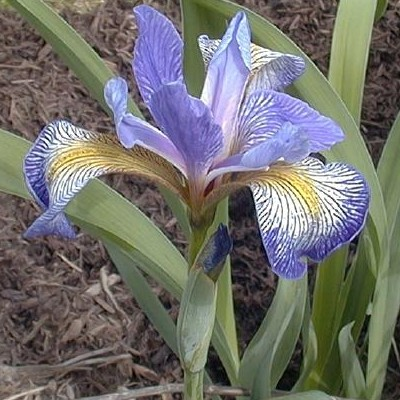
\includegraphics[width=3cm]{pics/virginica.jpg}
&
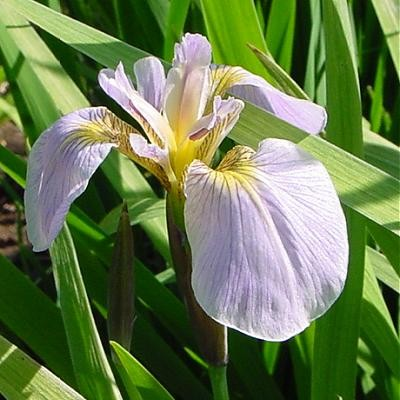
\includegraphics[width=3cm]{pics/setosa.jpg}
&
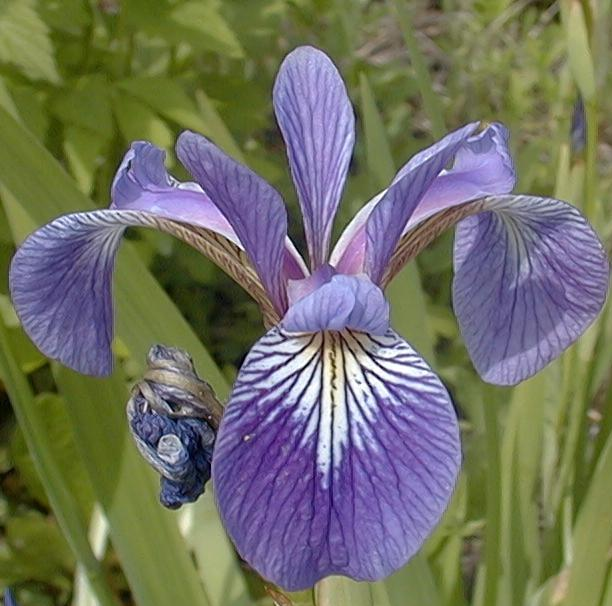
\includegraphics[width=3cm]{pics/versicolor.jpg}
\end{tabular}
\caption{Virginica - Setosa - Versicolor}
\end{center}
\end{figure}

\begin{itemize}
 \item The dataset is available in R:
 \begin{verbatim}
>data(iris) #  to load the dataset into the workspace
> names(iris)
[1] "Sepal.Length" "Sepal.Width"  "Petal.Length" 
		    "Petal.Width"  "Species"     
 \end{verbatim}

 \item In order to access the variables directly in our workspace we use the command \verb+attach(iris)+.
 
 
\end{itemize}



}

\end{frame}




\section{Summary Statistics}
\begin{frame}[fragile]{Summary Statistics}
\scriptsize{
\begin{itemize}
\item Summary statistics are values that explain properties of the data.
 \item Some of these properties include: frequencies, measures of central tendency and dispersion.
 \item Example: 
 \begin{itemize}
  \scriptsize{
  \item Central tendency: mean, median, mode.
  \item Variation: measure the variability of the data, such as standard deviation, range, etc..
 }
 \end{itemize}
 
 \item Most summary statistics can be calculated by making a single pass through the data.

\end{itemize}



}
 
\end{frame}

\begin{frame}[fragile]{Frequency and Mode}
\scriptsize{
\begin{itemize}
 \item The absolute frequency of an attribute value is the number of times it is observed.
 \item The relative frequency is the absolute frequency divided by the total number of examples.
 \item In R we can count the frequencies of occurrence of each distinct value of a vector using the command \verb+table+: 
 \begin{verbatim}
> table(iris$Species)
    setosa versicolor  virginica 
        50         50         50  
> vec<-c(1,1,1,0,0,3,3,3,3,2)
> table(vec)
vec
0 1 2 3 
2 3 1 4 
 \end{verbatim} 
 \item Exercise: Calculate the relative frequencies of the above vector. 
 \begin{verbatim}
> table(vec)/length(vec)  # Relative frequencies
vec
  0   1   2   3 
0.2 0.3 0.1 0.4   
\end{verbatim}

 

\end{itemize}

 
 
} 
\end{frame}

\begin{frame}[fragile]{Frequency and Mode (2)}
\scriptsize{
\begin{itemize}
 \item The mode of an attribute is the most frequent value observed.
 \item The mode function is not implemented natively in R, but it is easy to calculate using \verb+table+ and \verb+max+:
 \begin{verbatim}
my_mode<-function(var){
  frec.var<-table(var)
  value<-which(frec.var==max(frec.var))
  as.numeric(names(value))
}
> my_mode(vec)
[1] 3
> my_mode(iris$Sepal.Length)
[1] 5
 \end{verbatim}
 
\item We generally use frequencies and mode to study categorical variables.

\end{itemize}
 

 }
\end{frame}


\begin{frame}[fragile]{Central Tendency Measures}
\scriptsize{
\begin{itemize}
 \item These measures attempt to summarize the observed values into a single value associated with the centrally located value.
 \item The mean is the most common measure of central tendency for a numeric variable.  
 \item If we have $n$ observations it is calculated as the arithmetic mean or average.
 \begin{displaymath}
   \text{mean}(x) = \overline{x} = \frac{1}{n} \sum_{i=1}^{n} x_i
 \end{displaymath}

 \item The major problem with the mean is that it is very sensitive to \textbf{outliers}.
 
 \item We take a random vector of mean $20$ and then add a random element that comes from a distribution of much larger mean.  We see that the mean is strongly affected by noise:
 \begin{verbatim}
> vec<-rnorm(10,20,10)
> mean(vec)
[1] 16.80036
> vec.noise<-c(vec,rnorm(1,300,100))
> mean(vec.noise)
[1] 35.36422
 \end{verbatim}

 
\end{itemize}

 
}
 
\end{frame}

\begin{frame}[fragile]{Central Tendency Measures (2)}
\scriptsize{
\begin{itemize}
 \item We can robust the mean by removing a fraction of the extreme values using the \textbf{trimmed mean}.
 \item In R we can give a second parameter to the function \verb+mean+ called \verb+trim+ that defines the fraction of extreme elements to discard. 
 \item Example: We discard $10\%$ of the extreme values in the previous example:
 \begin{verbatim}
> mean(vec,trim=0.1)
[1] 17.78799
> mean(vec.noise,trim=0.1)
[1] 19.51609  # much more robust  
\end{verbatim}

 
\end{itemize}

 
}
 
\end{frame}


\begin{frame}[fragile]{Central Tendency Measures (3)}
\scriptsize{
\begin{itemize}
 \item The median represents the central ranking position of the variable that separates the lower half and the upper half of the observations.
 \item Intuitively, it consists of the value where for one half of the observations all values are greater than it, and for the other half all are less.
   \begin{displaymath}
  \text{median}(x) =  \left\{ \begin{array}{rl}
    x_{r+1} &\mbox{ If $|x|$ (vector length) is odd, $|x|=2r+1$} \\
   \frac{1}{2}(x_r + x_{r+1}) &\mbox{ If $|x|$ is even, $|x|=2r$ }
       \end{array} \right.
  \end{displaymath}
 
 \item For the above example, we see that the median is more robust to noise than the mean:
 \begin{verbatim}
> median(vec)
[1] 17.64805
> median(vec.noise)
[1] 17.64839
 \end{verbatim}

 
\end{itemize}

 
}
 
\end{frame}

\begin{frame}{Comparison between mode, median and mean}
 
 \begin{figure}[h!]
	\centering
	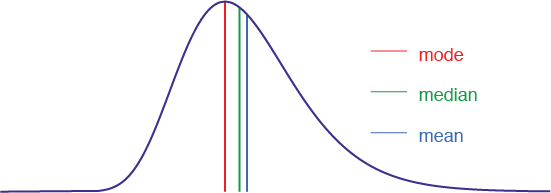
\includegraphics[scale=0.5]{pics/centrales.png}
	
	
\end{figure}
 
\end{frame}







\begin{frame}[fragile]{Percentiles or Quantiles}
\scriptsize{
\begin{itemize}
 \item The $k$-th percentile of a numerical variable is a value such that $k\%$ of the observations are below the percentile and $(100-k)\%$ are above this value.
 
 \item Quantiles are equivalent to percentiles but expressed in fractions instead of percentages. 
 
 \item In R they are calculated with the command \verb+quantile+:
 \begin{verbatim}
# All percentiles
quantile(Sepal.Length,seq(0,1,0.01))
 \end{verbatim}

 
 \item In addition it is very common to talk about the \textbf{quartiles} which are three specific percentiles:
 
 \begin{itemize}
 \scriptsize{
  \item The first quartile $Q_1$ (lower quartile) is the percentile with $k=25$. 
  \item The second quartile $Q_2$ is with $k=50$ which is equivalent to the median. 
  \item The third quartile $Q_3$ (upper quartile) is with $k=75$.
  }
 \end{itemize}
\begin{verbatim}
# The minimum, the three quartiles and the maximum.
> quantile(Sepal.Length,seq(0,1,0.25))
  0%  25%  50%  75% 100% 
 4.3  5.1  5.8  6.4  7.9  
\end{verbatim}

 
\end{itemize}

}

 
\end{frame}


\begin{frame}[fragile]{Summarizing a Data Frame}
\scriptsize{
\begin{itemize}
 \item In R we can summarize various summary statistics of a variable or of a data.frame using the command \verb+summary+.
 \item For numerical variables it gives us the minimum, the quartiles, the mean and the maximum.  
 \item For categorical variables it gives us the frequency table.
\end{itemize}


\begin{verbatim}
> summary(iris)
 Sepal.Length    Sepal.Width     Petal.Length    Petal.Width   
 Min.   :4.300   Min.   :2.000   Min.   :1.000   Min.   :0.100  
 1st Qu.:5.100   1st Qu.:2.800   1st Qu.:1.600   1st Qu.:0.300  
 Median :5.800   Median :3.000   Median :4.350   Median :1.300  
 Mean   :5.843   Mean   :3.057   Mean   :3.758   Mean   :1.199  
 3rd Qu.:6.400   3rd Qu.:3.300   3rd Qu.:5.100   3rd Qu.:1.800  
 Max.   :7.900   Max.   :4.400   Max.   :6.900   Max.   :2.500  

 Species  
 setosa    :50  
 versicolor:50  
 virginica :50   
\end{verbatim}

 
} 
\end{frame}


\begin{frame}[fragile]{Exercise}
\scriptsize{
\begin{itemize}
\item Using the command \verb+tapply+ analyze the mean, median and quartiles for the three species of \textbf{Iris} for the four variables.
 \item Do you notice any differences in the different species?
\end{itemize}


\begin{verbatim}
tapply(iris$Petal.Length,iris$Species,summary)
tapply(iris$Petal.Width,iris$Species,summary)
tapply(iris$Sepal.Length,iris$Species,summary)
tapply(iris$Sepal.Width,iris$Species,summary) 
\end{verbatim}


} 
\end{frame}

\begin{frame}[fragile]{Variability Measures}
\scriptsize{ 
\begin{itemize}
 \item Variability mesaures or dispersion measures tell us how different or similar the observations tend to be with respect to a particular value. Usually this value refers to some measure of central tendency.
 \item  The range is the difference between the maximum and minimum value:
 \begin{verbatim}
> max(Sepal.Length)-min(Sepal.Length)
[1] 3.6
 \end{verbatim}
 \item The standard deviation is the square root of the variance that measures the mean squared differences of the observations from the mean.  
 \begin{displaymath}
  \text{var}(x)=\frac{1}{n-1}\sum_{i=1}^{n}(x_{i} - \overline{x} )^2
 \end{displaymath}
 \begin{displaymath}
  \text{sd}(x)=\sqrt{\text{var}(x)}
 \end{displaymath}

\begin{verbatim}
> var(Sepal.Length)
[1] 0.6856935
> sd(Sepal.Length)
[1] 0.8280661 
\end{verbatim}



\end{itemize}
 
 
 
} 
\end{frame}


\begin{frame}[fragile]{Variability Measures (2)}
\scriptsize{ 
\begin{itemize}
 \item Like the mean, the standard deviation is sensitive to outliers.
 \item The most robust measures are usually based on the median.

  \item Let $m(x)$ be a measure of central tendency of $x$ (usually the median), we define the \textbf{average absolute deviation} (AAD)  as:
  \begin{displaymath}
   \text{AAD}(x) = \frac{1}{n}\sum_{i=1}^{n}|x_i-m(x)| 
  \end{displaymath}
  
  \item Exercise: Program the function \verb+add+ in R, as a function that receives a vector \verb+x+ and a central mean function \verb+fun+. The absolute value is calculated with the command \verb+abs+:
  
  \begin{verbatim}
aad<-function(x,fun=median){
  mean(abs(x-fun(x)))
}
> aad(Sepal.Length)
[1] 0.6846667
> aad(Sepal.Length,mean)
[1] 0.6875556
  \end{verbatim}


\end{itemize}
 
 
 
} 
\end{frame}


\begin{frame}[fragile]{Variability Measures (3)}
\scriptsize{ 
\begin{itemize}
 \item Let $b$ be a constant we define the \textbf{mean absolute deviation} as: 
 \begin{displaymath}
  \text{MAD}(x) = b \times \text{median}(|x_{i}-\text{m}(x)|)
 \end{displaymath}
 \item In R is calculated with the command \verb+mad+ with the parameters \verb+center+ as a function measuring the central tendency of the variable and \verb+constant+ as the constant $b$. By default the median and the value $1.482$ is used. 
 \begin{verbatim}
 > mad(Sepal.Length)
[1] 0.7 
 \end{verbatim}

 \item Finally, the interquartile range (IQR) is defined as the difference between the third and the first quartile ($Q_3 - Q_1$).
 \begin{verbatim}
IQR(Sepal.Length)
[1] 1.3  
 \end{verbatim}

\end{itemize}
  
} 
\end{frame}



\begin{frame}[fragile]{Multivariate Summary Statistics}
\scriptsize{
\begin{itemize}
 \item To compare how one variable varies with respect to another, we use multivariate measures.
 \item The covariance $cov(x,y)$ measures the degree of joint linear variation of a pair of variables $x$, $y$:
 \begin{displaymath}
  cov(x,y)=\frac{1}{n-1}\sum_{i=1}^{n}(x-\overline{x})(y-\overline{y})
 \end{displaymath}
 \item Where $cov(x,x)=var(x)$
\item In R it is computed with the command  \verb+cov+:
\begin{verbatim}
> cov(Sepal.Length,Sepal.Width)
[1] -0.042434 
\end{verbatim}
\item If we give it a matrix or a data.frame of numeric variables, it computes a covariance matrix:
\begin{verbatim}
> cov(iris[,1:4])
             Sepal.Length Sepal.Width Petal.Length Petal.Width
Sepal.Length    0.6856935  -0.0424340    1.2743154   0.5162707
Sepal.Width    -0.0424340   0.1899794   -0.3296564  -0.1216394
Petal.Length    1.2743154  -0.3296564    3.1162779   1.2956094
Petal.Width     0.5162707  -0.1216394    1.2956094   0.5810063 
\end{verbatim}

 
 
 
\end{itemize}



}
\end{frame}


\begin{frame}[fragile]{Multivariate Summary Statistics (2)}
\scriptsize{
\begin{itemize}
 \item If two variables are independent of each other, their covariance is zero.
 \item A measure of relationship that does not depend on the scale of each variable is the \textbf{linear correlation}.
 \item The linear correlation or \textbf{Pearson's} correlation coefficient $r(x,y)$ is defined as: 
 \begin{displaymath}
  r(x,y)=\frac{cov(x,y)}{sd(x)sd(y)}
 \end{displaymath}
\item  The linear correlation varies between $-1$ to $1$. 

\end{itemize}



}
\end{frame}



\begin{frame}[fragile]{Multivariate Summary Statistics (3)}
\scriptsize{
\begin{itemize}
\item A value close to 1 indicates that as one variable grows the other also grows in a linear proportion. 
\item A value close to -1 indicates an inverse relationship (one is growing and the other is decreasing). 
\item If the correlation is close to zero we have linear independence. 
\item Note that a correlation of zero does not imply that there cannot be a non-linear relationship between the variables.
\item In R, the correlation is calculated with the command \verb+cor+.
\begin{verbatim}
> cor(iris[,1:4])
             Sepal.Length Sepal.Width Petal.Length Petal.Width
Sepal.Length    1.0000000  -0.1175698    0.8717538   0.8179411
Sepal.Width    -0.1175698   1.0000000   -0.4284401  -0.3661259
Petal.Length    0.8717538  -0.4284401    1.0000000   0.9628654
Petal.Width     0.8179411  -0.3661259    0.9628654   1.0000000
\end{verbatim}

 
 
\end{itemize}



}
\end{frame}


\begin{frame}[fragile]{Contingency Tables}
\scriptsize{
\begin{itemize}
 \item To analyze the relationship between categorical variables  we use \textbf{contingency tables}.
 \item The table is filled with the marginal frequencies of all pairs of values between two categorical variables.
 \item In R they are created using the command \verb+table+ that we used before for computing frequencies, but now giving two vectors as input:
 \begin{verbatim}
gender<-c("Male", "Female", "Male", "Female", "Female", "Male")
studies<-c("college","postgraduate","high school",
            "postgraduate","high school","college")
            
>table(gender,studies)
        studies
gender   college high school postgraduate
  Female       0           1            2
  Male         2           1            0
 \end{verbatim}

 
 
\end{itemize}


} 
\end{frame}


\begin{frame}{Skweness and Kurtosis}
\scriptsize{
There are other two summary statistics that focus on more complex properties of the data distribution called skeweness and kurtosis \cite{pipis_2020}.
\begin{block}{Skeweness}
\begin{itemize}
 \item Skeweness is a measure of the \textbf{asymmetry} of the probability distribution.  
 \begin{displaymath}
  \text{skewness}(x) = \frac{\sum_{i=1}^{n}(x_i-\overline{x})^3}{(n-1)sd(x)^3}
 \end{displaymath}

 
 \item It indicates how much our underlying distribution deviates from the normal distribution since the normal distribution has skewness 0.
 \item  Generally, we have three types of skewness:
 
 \begin{enumerate}
 \scriptsize{
  \item     \textbf{Symmetrical}: the skewness is close to 0 and the mean is almost the same as the median.
  \item \textbf{Negative skew}: the majority of the observations are concentrated on the right tail (the median is greater than the mean).
  \item  \textbf{Positive skew}: the majority of the observations are concentrated on the left tail (the median is less than the mean). }
 \end{enumerate}

\end{itemize}


\end{block}




}
 
\end{frame}


\begin{frame}{Skweness}


   \begin{figure}[h!]
	\centering
	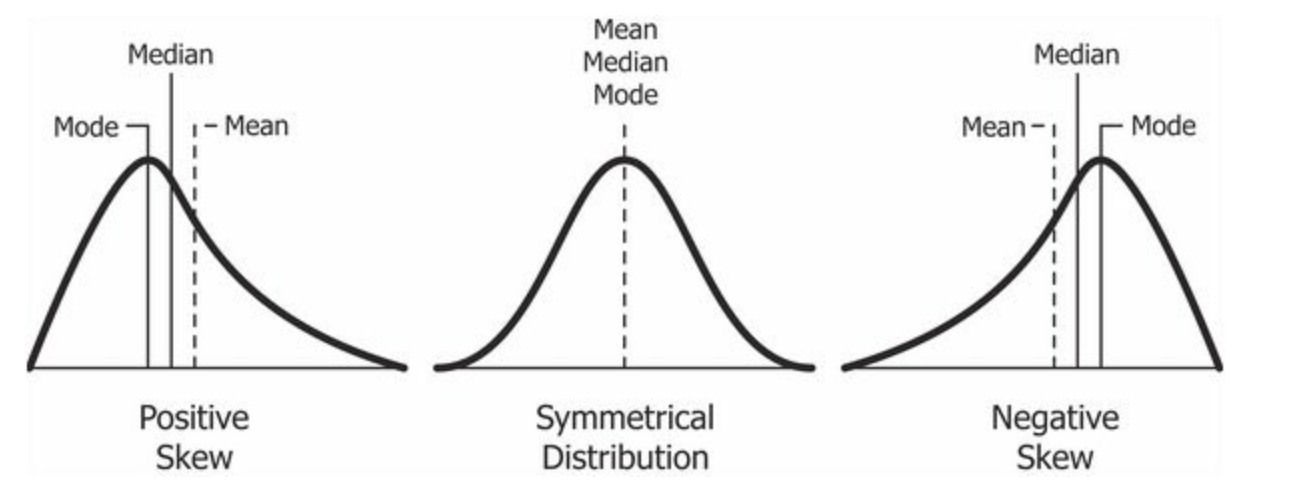
\includegraphics[scale=0.68]{pics/skewness.png}
     \caption{Source: Wikipedia}
	\end{figure} 




 
\end{frame}


\begin{frame}[fragile]{Skweness}

\scriptsize{
\begin{itemize} 
 \item In R, we can calculate skweness with the formula \textbf{skewness} from the library \textbf{moments}:
 
 \begin{verbatim}
> library(moments)
#positive skew
> skewness(c(1,1,2,3)) 
[1] 0.4933822
#symmetrical
> skewness(c(1,2,3)) 
[1] 0
#negative skew
> skewness(c(1,2,3,3)) 
[1] -0.4933822
 \end{verbatim}

 
 
\end{itemize}

}



 
\end{frame}


\begin{frame}{Kurtosis}
\scriptsize{


\begin{block}{Kurtosis}
\begin{itemize}
 \item The Kurtosis  describes the ``tailedness'' of a distribution \cite{westfall2014kurtosis}. 
 
  \begin{displaymath}
  \text{kurtosis}(x) = \frac{\sum_{i=1}^{n}(x_i-\overline{x})^4}{(n-1)sd(x)^4}
 \end{displaymath}
 
  \item  Let's see the main three types of kurtosis.
 
 \begin{enumerate}
 \scriptsize{
   \item  \textbf{Mesokurtic}: This is the normal distribution (kurtosis $\approx 3$)
    \item \textbf{Leptokurtic}: This distribution has fatter tails than a normal distribution (kurtsosis $> 3$). Consequently, outliers are more likely to occur than in a normal distribution.
    \item \textbf{Platykurtic}: The distribution has thinner tails than a normal distribution (kurtosis $< 3$). Consequently, outliers are less likely to occur than in a normal distribution.}
 \end{enumerate}

 
 
\end{itemize}



\end{block}


}
 
\end{frame}


\begin{frame}{Kurtosis}



   \begin{figure}[h!]
	\centering
	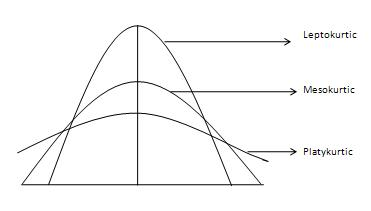
\includegraphics[scale=0.9]{pics/kurtosis.jpg}
     \caption{Source: tutorialspoints}
	\end{figure} 
 
 




 
\end{frame}

\begin{frame}[fragile]{Kurtosis}

\scriptsize{
\begin{itemize} 
 \item In R, we can calculate kurtosis with the formula \textbf{kurtosis} from the library \textbf{moments}.
 
 \item Let's calculate kurtosis for normal data:
 
 \begin{verbatim}
> x <- rnorm(1000, 0,1)
> plot(density(x))
> kurtosis(x)
[1] 2.946869
 \end{verbatim}

 \item  As expected we got a value close to 3.

 
   \begin{figure}[h!]
	\centering
	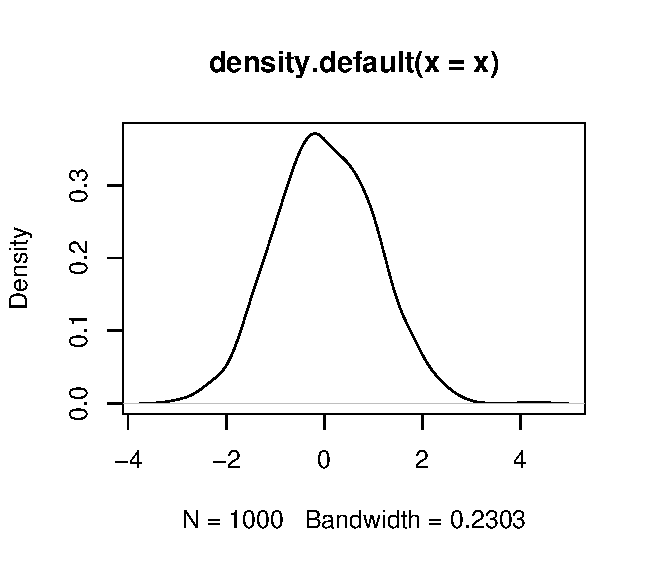
\includegraphics[scale=0.4]{pics/kurt1.pdf}
	\end{figure} 
 
 
 
\end{itemize}

}

 
\end{frame}


\begin{frame}[fragile]{Kurtosis}

\scriptsize{
\begin{itemize} 
 \item Now using random data generated with an exponential long-tailed distribution:
 
 \begin{verbatim}
> x<-rexp(1000)
> plot(density(x))
> kurtosis(x)
[1] 6.839485
 \end{verbatim}

 \item  As expected we get a positive excess kurtosis (i.e. greater than 3) since the distribution has fatter tails (Leptokurtic).

 
   \begin{figure}[h!]
	\centering
	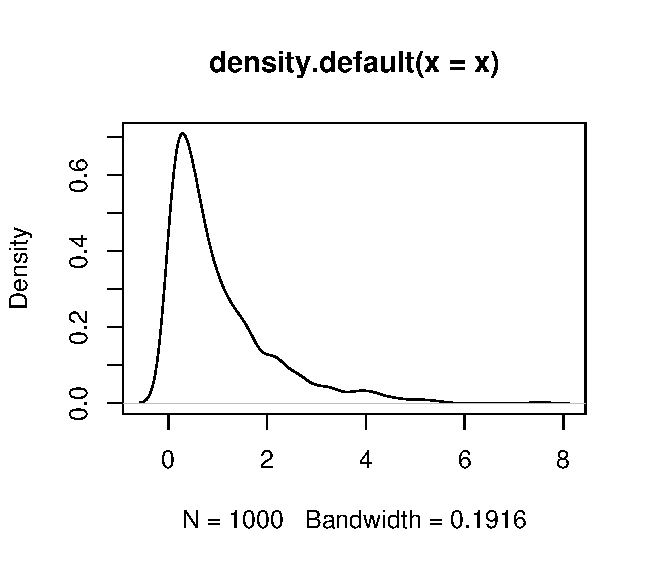
\includegraphics[scale=0.4]{pics/kurt2.pdf}
	\end{figure} 
 
 
 
\end{itemize}

}

 
\end{frame}



\begin{frame}[fragile]{Kurtosis}

\scriptsize{
\begin{itemize} 
 \item Now using data generated with a thinner-tailed Beta distribution with hyperparameters $5,5$:
 
 \begin{verbatim}
> x <-rbeta(1000,2,2)
> plot(density(x))
> kurtosis(x)
[1] 2.1046
 \end{verbatim}

 \item  As expected we get a negative excess kurtosis (i.e. less than 3) since the distribution has thinner tails (Platykurtic). 
 
   \begin{figure}[h!]
	\centering
	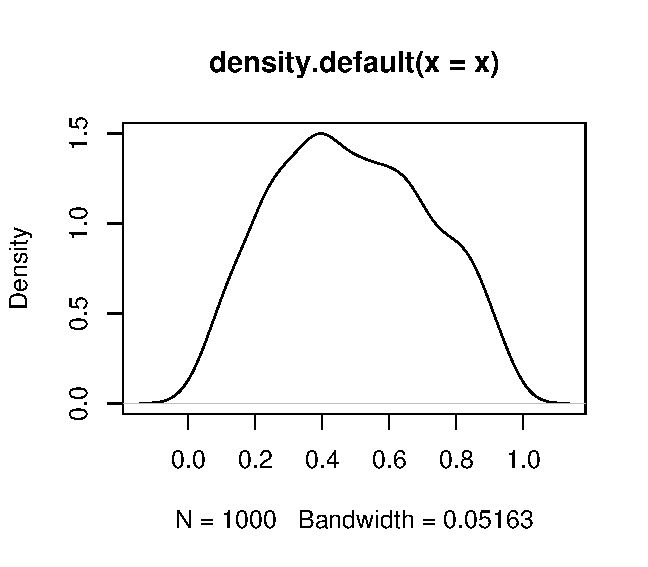
\includegraphics[scale=0.4]{pics/kurt3.pdf}
	\end{figure} 
 
 
 
\end{itemize}

}

 
\end{frame}


\section{Visualization}


\begin{frame}[fragile]{Data Visualization}
\scriptsize{
\begin{itemize} 
 \item Data visualization is the transformation of a dataset into a visual format that allows people to identify the characteristics and relationships between examples in the dataset.
 
 \item Visualization allows people to recognize patterns or trends based on their judgment or expertise in the particular domain.
 
   \begin{figure}[h!]
	\centering
	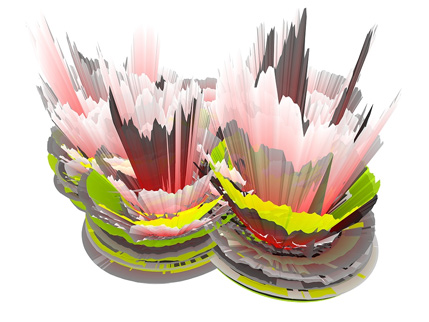
\includegraphics[scale=0.38]{pics/visua.jpg}
	
	
\end{figure} 
 
\end{itemize}

}
 
\end{frame}

\begin{frame}{Representation}
\scriptsize{
\begin{itemize}
 \item Representation is understood as the mapping of data into a visual format
 \item Examples, their attributes and relationships are translated into graphical elements such as points, lines, shapes and colors.  
  \item Examples are usually represented as points.
  \item Attribute values are represented as the position of the points or the characteristics of the points, e.g. color, size and shape.
  \item When using position to represent values it is simple to detect if groups of objects are formed or the presence of outliers. 
  
 
 
\end{itemize}
 
 

 
}
\end{frame}


\begin{frame}[fragile]{Plotting in R}
\scriptsize{
\begin{itemize}
 \item  In R the most frequent display function is \verb+plot+. 
 \item t is a generic function whose result depends on the nature of the variables given as input.  
 
 \item  To all plots we can add additional parameters such as: \verb+main+ for the title, \verb+xlab+ and \verb+ylab+ for the name of the x-axis and y-axis.
 
 \item Other properties are: \verb+col+ to define the color, \verb+type+ to define the chart type: (p) for points or (l) for lines.
 
 \item We can also add new layers to a plot with the command \verb+lines+.
 
 \item To save an image to a file we can use Rstudio's \textbf{export} button.
 
 \item To do it from the R command line:
 \begin{verbatim}
png("imagen.png")
plot(1:10)
dev.off() 
 \end{verbatim}

 


 
 
\end{itemize}


 
} 
\end{frame}


\begin{frame}[fragile]{Example}
\scriptsize{
  \begin{verbatim}
plot(rnorm(15,10,5),col="red",type="p",pch=1)
lines(rnorm(15,10,5),col="blue",type="p",pch=1)
lines(rnorm(15,10,5),col="green",type="b",pch=2)
title(main="My Plot")
legend('topright', c("lines","dots","both") , 
       lty=1:3, col=c("red", "blue","green"), bty='n', cex=.75)
\end{verbatim}
  
  \begin{figure}[h!]
	\centering
	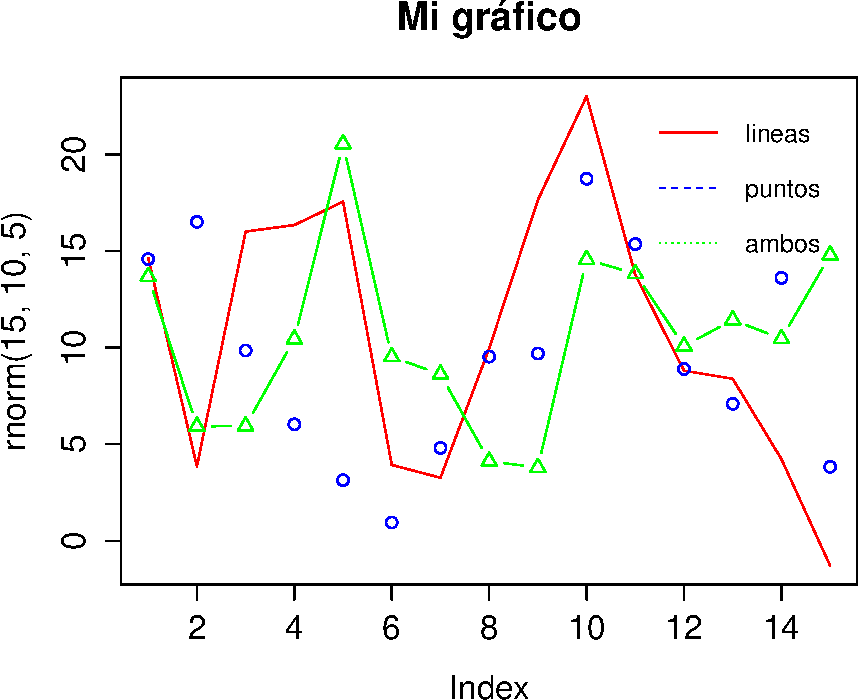
\includegraphics[scale=0.43]{pics/rplot.pdf}
	
	
\end{figure} 



 
} 
\end{frame}



\begin{frame}[fragile]{Histograms}
\scriptsize{
\begin{itemize}
 \item They show the distribution of the values of a variable.
 \item The values of the elements are divided into bins and bar charts are created for each of them.
 \item The height of each bar indicates the number of examples in the corresponding bin.
 \item In R they are created with the command \verb+hist+.
 \begin{verbatim}
> hist(Sepal.Length)
 \end{verbatim}
 \begin{figure}[h!]
	\centering
	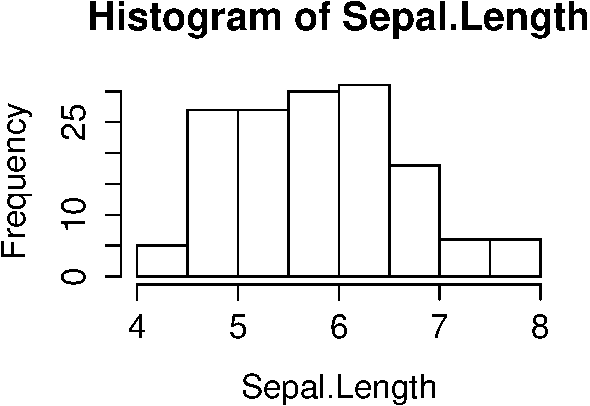
\includegraphics[scale=0.6]{pics/hist1.pdf}
	
	
\end{figure} 

\end{itemize}




}
\end{frame}


\begin{frame}[fragile]{Histograms (2) }
\scriptsize{
\begin{itemize}
 \item The shape of the histogram depends on the number of bins.
 \item In R this number can be defined with the parameter  \verb+nclass+.
 \begin{verbatim}
> hist(Sepal.Length,nclass=100)
 \end{verbatim}
 \begin{figure}[h!]
	\centering
	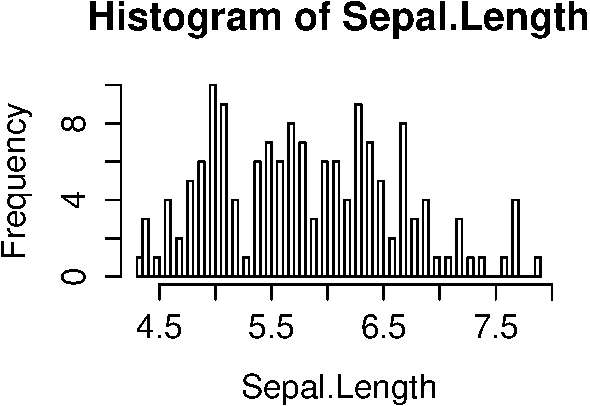
\includegraphics[scale=0.6]{pics/hist2.pdf}
	
	
\end{figure} 

\end{itemize}

}
\end{frame}


\begin{frame}[fragile]{Histograms (3) }
\scriptsize{
\begin{itemize}
 \item A very popular library for making visualizations in R, which is part of tidyverse, is \emph{ggplot2}.
 \item It is based on the idea of decomposing the plot into semantic components such as scales and layers.
 \begin{verbatim}
>install.packages("ggplot2")
>library(ggplot2)
>ggplot(iris, aes(x=Sepal.Length)) 
+ geom_histogram(bins = 10, color="black", fill="white")
 \end{verbatim}
 \begin{figure}[h!]
	\centering
	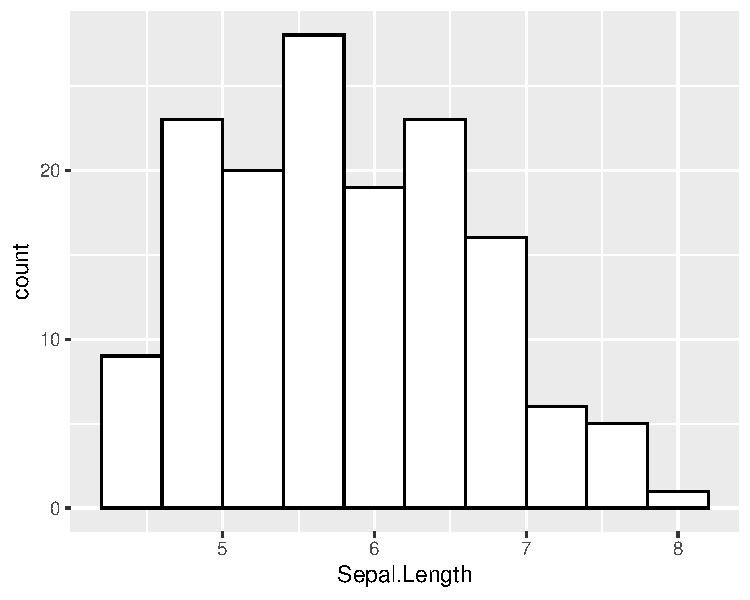
\includegraphics[scale=0.4]{pics/hist3.pdf}
	
	
\end{figure} 

\end{itemize}

}
\end{frame}


\begin{frame}[fragile]{Density}
\scriptsize{
\begin{itemize}
 \item Another way to visualize how the data are distributed is to estimate a density.
 \item These are calculated using nonparametric statistical techniques called \textbf{kernel} density estimation.
 \item The density is a smoothed version of the histogram and allows us to determine more clearly if the observed data behaves like a known density e.g. Gaussian.  
 \item In R they are created with the command \verb+density+, and then visualized with the command \verb+plot+.

 \begin{verbatim}
plot(density(iris$Sepal.Length),main=""Density of Sepal.Length")
 \end{verbatim}
 \begin{figure}[h!]
	\centering
	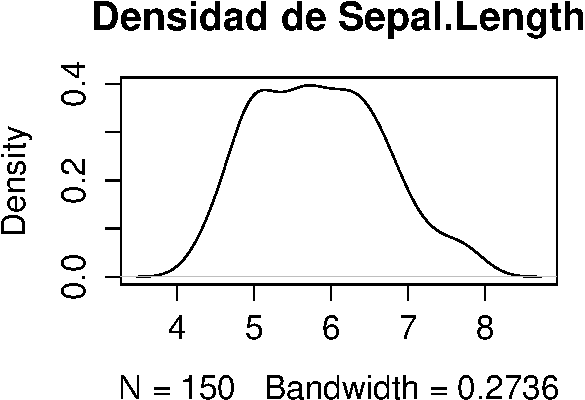
\includegraphics[scale=0.38]{pics/density.pdf}
	
	
\end{figure} 

\end{itemize}




}
\end{frame}


\begin{frame}[fragile]{Pie Charts }
\scriptsize{
\begin{itemize}
 \item The pie charts represent the frequency of the elements in a circle.
 \item Each category has a share proportional to its relative frequency.
 \item They are generally used for categorical variables:
 \begin{verbatim}
pie(table(iris$Species))
 \end{verbatim}
 \begin{figure}[h!]
	\centering
	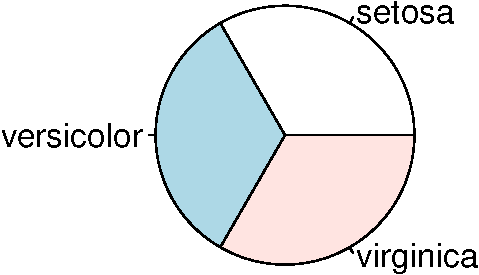
\includegraphics[scale=0.6]{pics/piechart.pdf}
	
	
\end{figure} 

\end{itemize}




}
\end{frame}


\begin{frame}[fragile]{Boxplots}
\scriptsize{
\begin{itemize}
 \item Boxplots are built from the percentiles. 
 \item A rectangle is constructed between the first and third quartiles ($Q_1$ and $Q_3$).
 \item The height of the rectangle is the interquartile range RIC ($Q_3 - Q_1$).
 \item The median is a line that divides the rectangle.
 \item Each end of the rectangle is extended with a line or arms of length $Q1-1.5*$IQR for the lower line and $Q_3+1.5*$IQR for the upper line.
 \item Values more extreme than the length of the arms are considered outliers.
 
 \item The boxplot gives us information about the symmetry of the data distribution.
  \item If the median is not in the center of the rectangle, the distribution is not symmetrical.
 \item They are useful to detect the presence of outliers.
 
\end{itemize}



}
\end{frame}


\begin{frame}{Boxplots (2)}
\begin{figure}[h!]
	\centering
	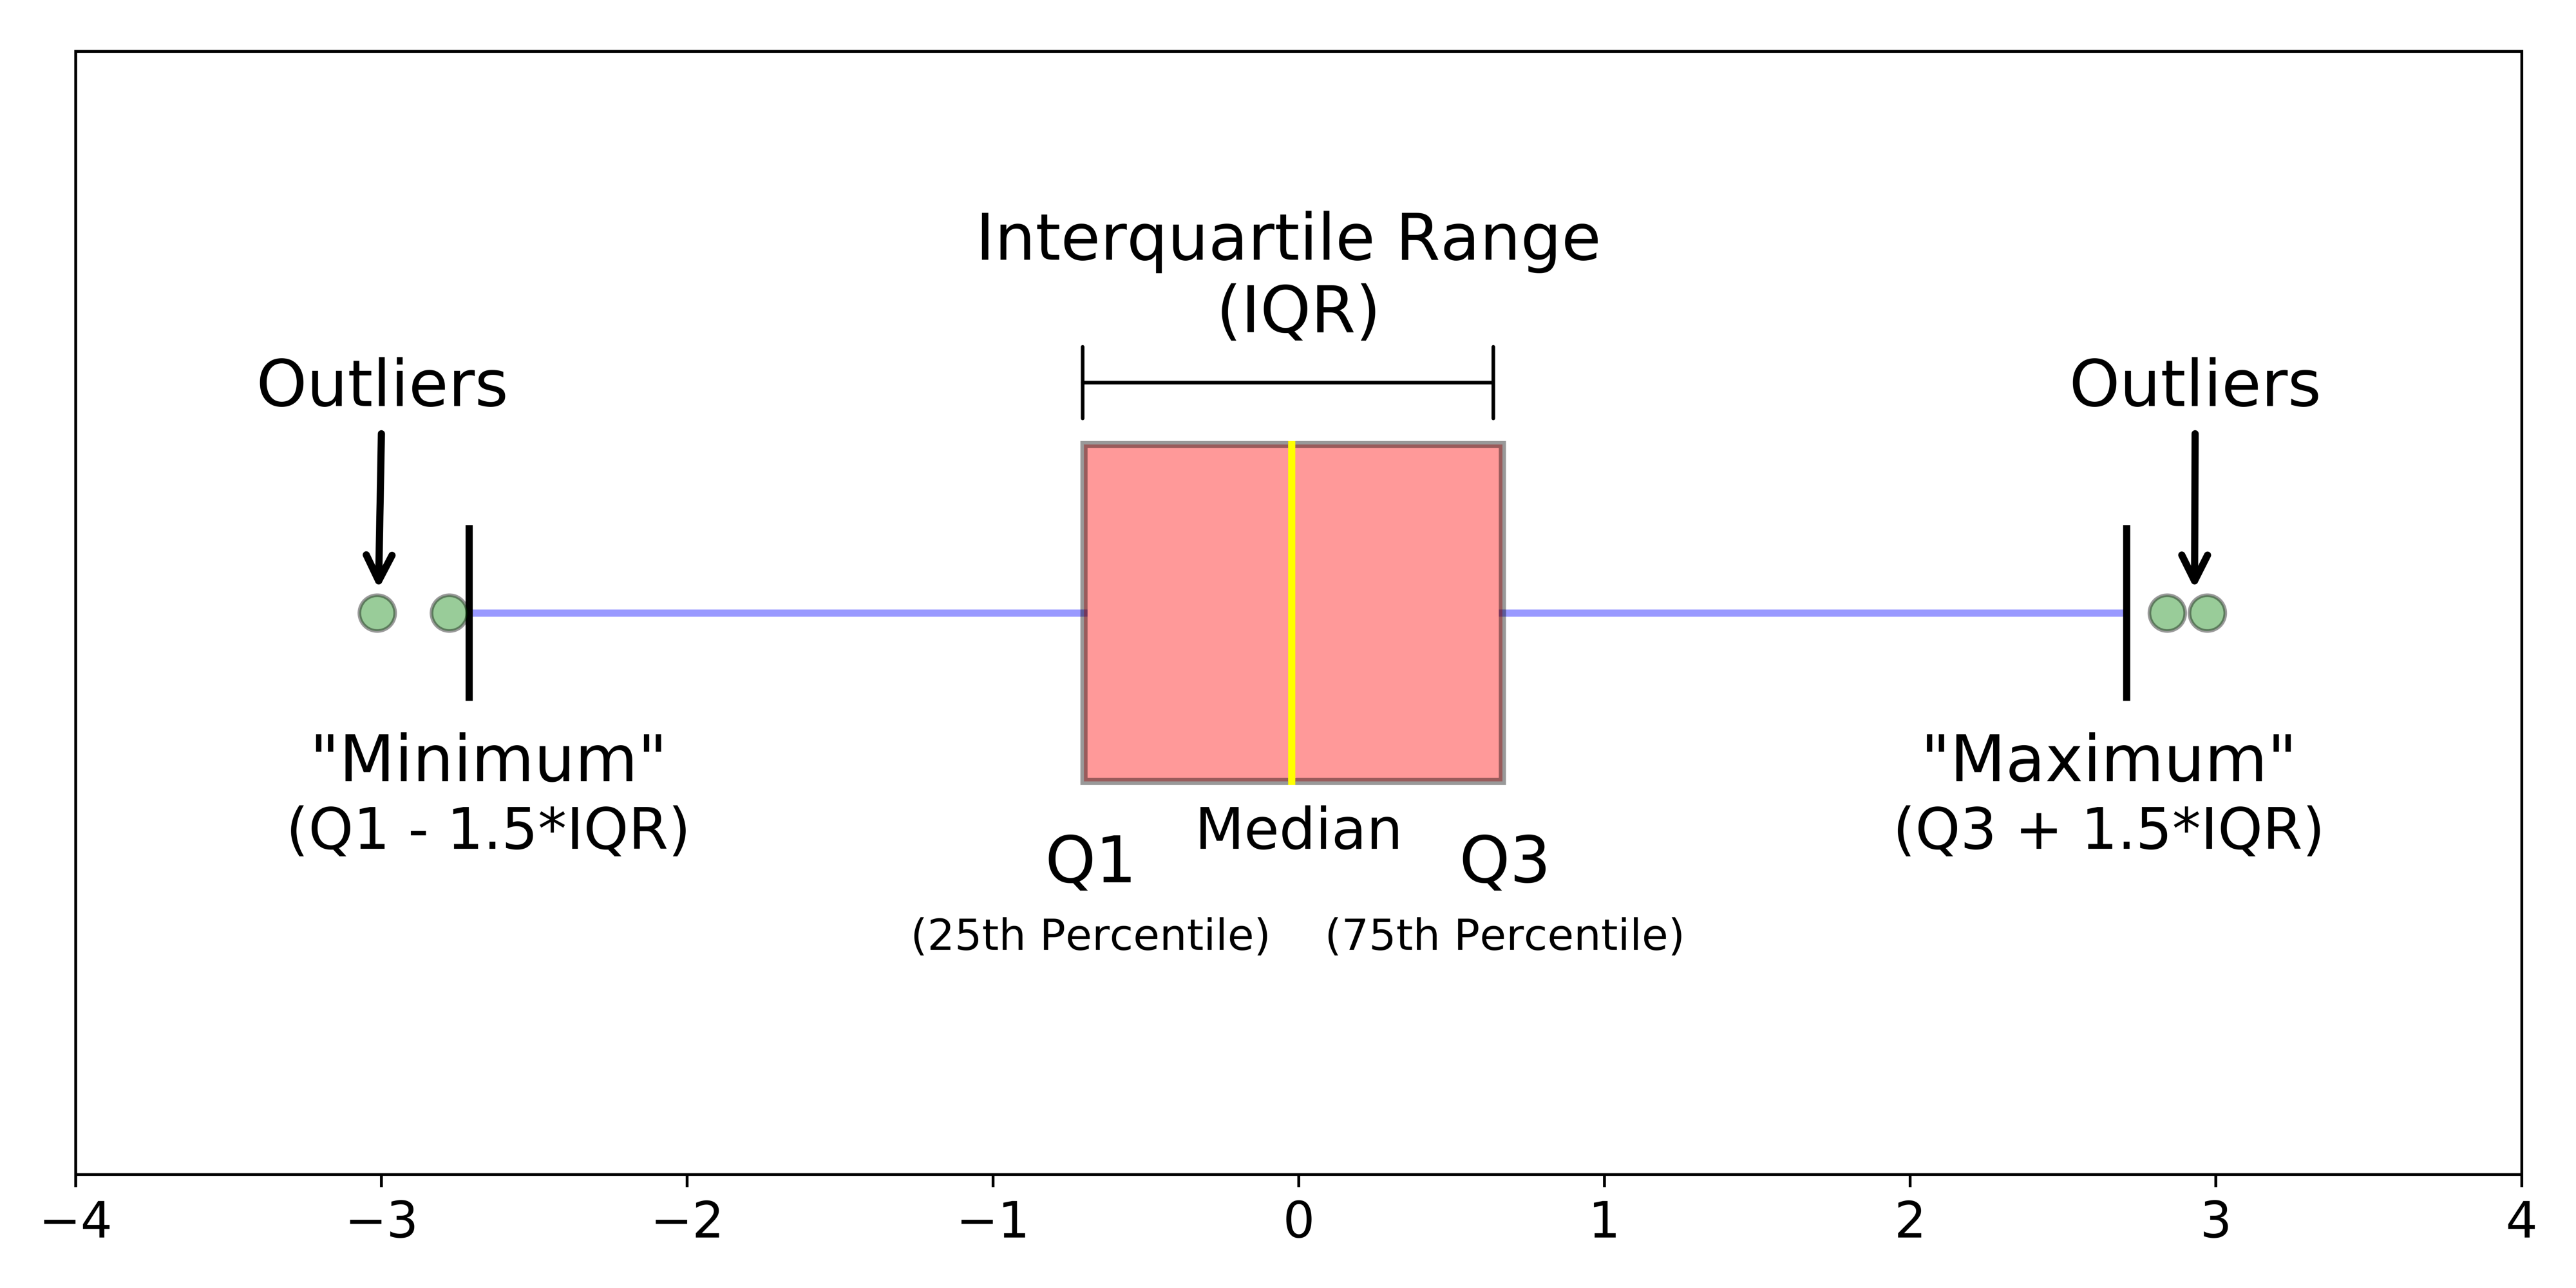
\includegraphics[scale=0.1]{pics/boxplot.png}
	\caption{\url{https://www.laboneconsultoria.com.br/wp-content/uploads/2018/07/Boxplot-04.png}}
	
\end{figure} 
\end{frame}


\begin{frame}{Boxplots (3)}
\scriptsize{
\begin{itemize}
 \item The length of the arms as well as the criteria for identifying outliers is based on the behavior of a normal distribution.
\end{itemize}

\begin{figure}[h!]
	\centering
	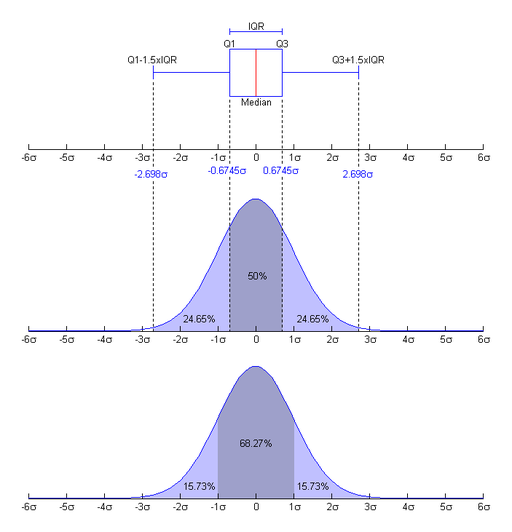
\includegraphics[scale=0.35]{pics/Boxplot_vs_PDF.png}
	
	
	
\end{figure} 
}
\end{frame}

\begin{frame}[fragile]{Boxplots (4)}
\scriptsize{
\begin{itemize}
 \item In R boxplots are plotted with the command \verb+boxplot+:
 \begin{verbatim}
> boxplot(Sepal.Length,main="Boxplot Sepal.Length")
 \end{verbatim}

 \begin{figure}[h!]
	\centering
	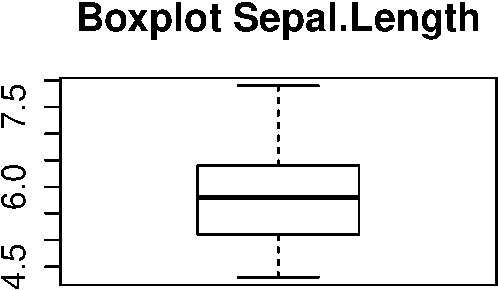
\includegraphics[scale=0.7]{pics/boxplotsimple.pdf}		
\end{figure} 
 
 
\end{itemize}



}
\end{frame}


\begin{frame}[fragile]{Boxplots (4)}
\scriptsize{
\begin{itemize}

\item If we have a factor variable we can create a boxplot for each category as follows:
\begin{verbatim}
> boxplot(Sepal.Length~Species,ylab="Sepal.Length")
\end{verbatim}

 \begin{figure}[h!]
	\centering
	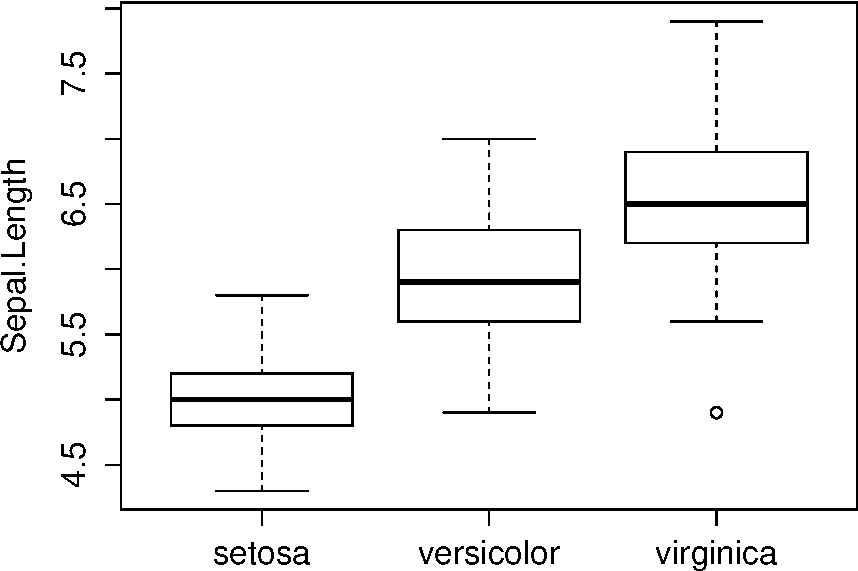
\includegraphics[scale=0.5]{pics/boxplotfactor.pdf}		
\end{figure} 
 
\end{itemize}

}
\end{frame}
\begin{frame}[fragile]{Boxplots (5)}
\scriptsize{
\begin{itemize}

\item We can also compare several boxplots in the same plot:
\begin{verbatim}
> boxplot(x=iris[,1:4],main="Boxplots Iris")
\end{verbatim}

 \begin{figure}[h!]
	\centering
	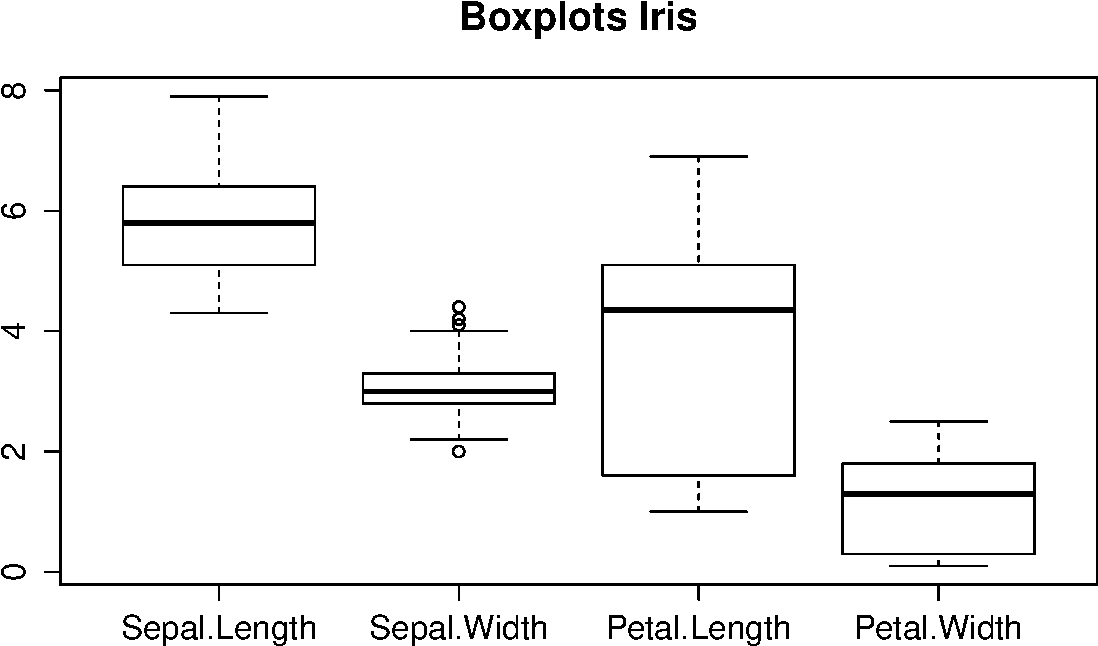
\includegraphics[scale=0.5]{pics/boxplotiris.pdf}		
\end{figure} 
 
\end{itemize}

}
\end{frame}



\begin{frame}[fragile]{Boxplots (6)}
\scriptsize{
\begin{itemize}

\item Now using \emph{ggplot2}:
\begin{verbatim}
> ggplot(iris, aes(x = Species, y = Sepal.Length, 
  fill = Species)) +  geom_boxplot()
\end{verbatim}

 \begin{figure}[h!]
	\centering
	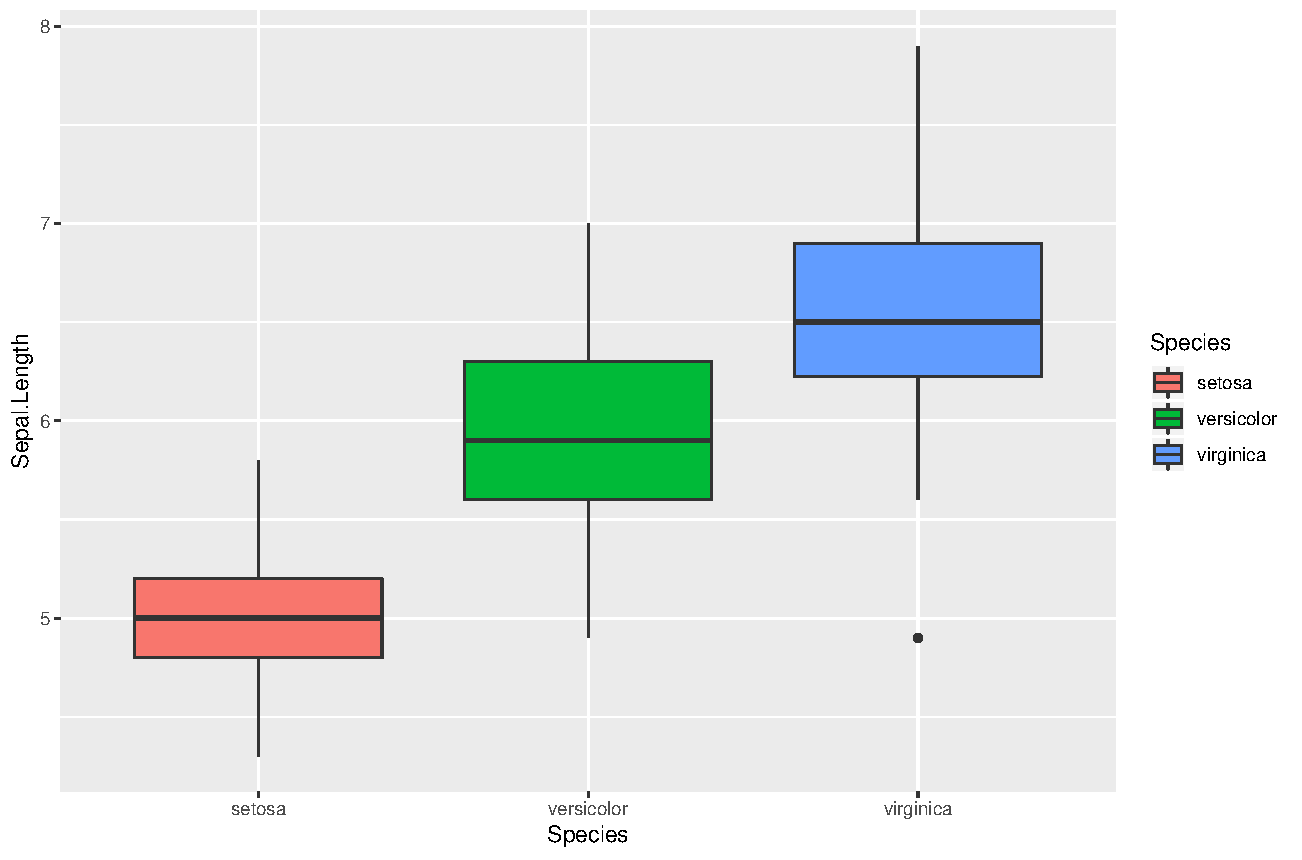
\includegraphics[scale=0.4]{pics/boxplotggplot2.pdf}		
\end{figure} 
 
\end{itemize}

}
\end{frame}


\begin{frame}[fragile]{Scatter Plots}
\scriptsize{
\begin{itemize}
 \item Scatter plots use Cartesian coordinates to display the values of two numerical variables of the same length.
 \item The values of the attributes determine the position of the elements.
 \item Other attributes can be used to define the size, shape or color of objects.
 
  \item In R we can plot a scatterplot of two numeric variables using the command \verb+plot(x,y)+, which would be $y$ vs $x$.
  
  \item We can also define formulas $f(x)=y$ using the notation \verb+y~x+.  
  
 \item Thus, the command \verb+plot(y~x)+ is equivalent to \verb+plot(x,y)+.
 
 \item If we have a data.frame or a numerical matrix, we can see the scatterplots of all pairs using the command \verb+pairs(x)+.
  
 
 
\end{itemize}




}
 
\end{frame}


\begin{frame}[fragile]{Scatter Plots (2)}
\scriptsize{
\begin{itemize}
 \item Examples:
 \begin{verbatim}
# Sepal width vs. sepal length 
plot(Sepal.Width~Sepal.Length, col=Species)
# Equivalent
plot(Sepal.Length, Sepal.Width,col=Species,
     pch=as.numeric(Species))
# We add a legend
legend('topright', levels(Species) , 
       lty=1, col=1:3, bty='n', cex=.75)  
 \end{verbatim}

  \begin{figure}[h!]
	\centering
	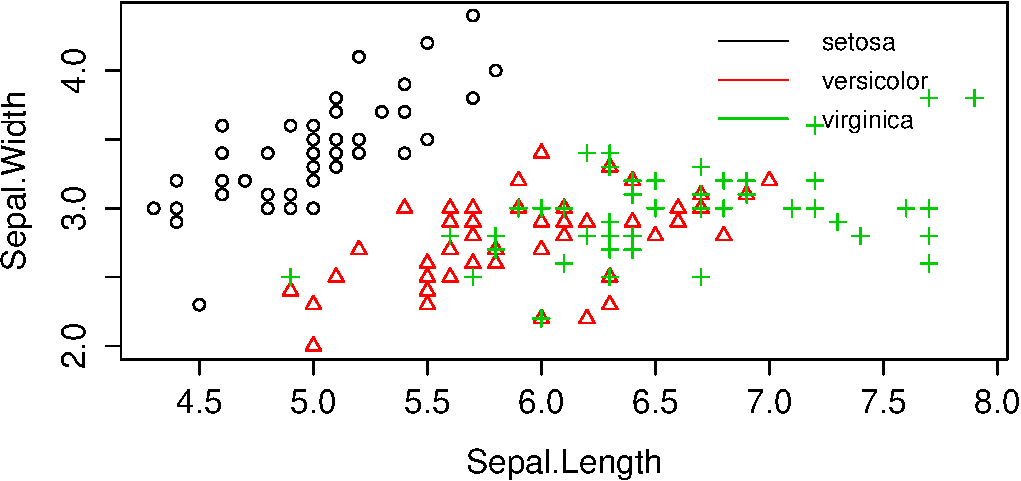
\includegraphics[scale=0.45]{pics/scatter1.pdf}		
\end{figure} 
 
 
\end{itemize}




}
 
\end{frame}


\begin{frame}[fragile]{Scatter Plots (3)}
\scriptsize{
\begin{itemize}
 \item The same using \emph{ggplot2}:
 \begin{verbatim}
ggplot(iris, aes(x=Sepal.Length,
y=Sepal.Width, color=Species)) + 
geom_point(size=3,shape=4)
 \end{verbatim}

  \begin{figure}[h!]
	\centering
	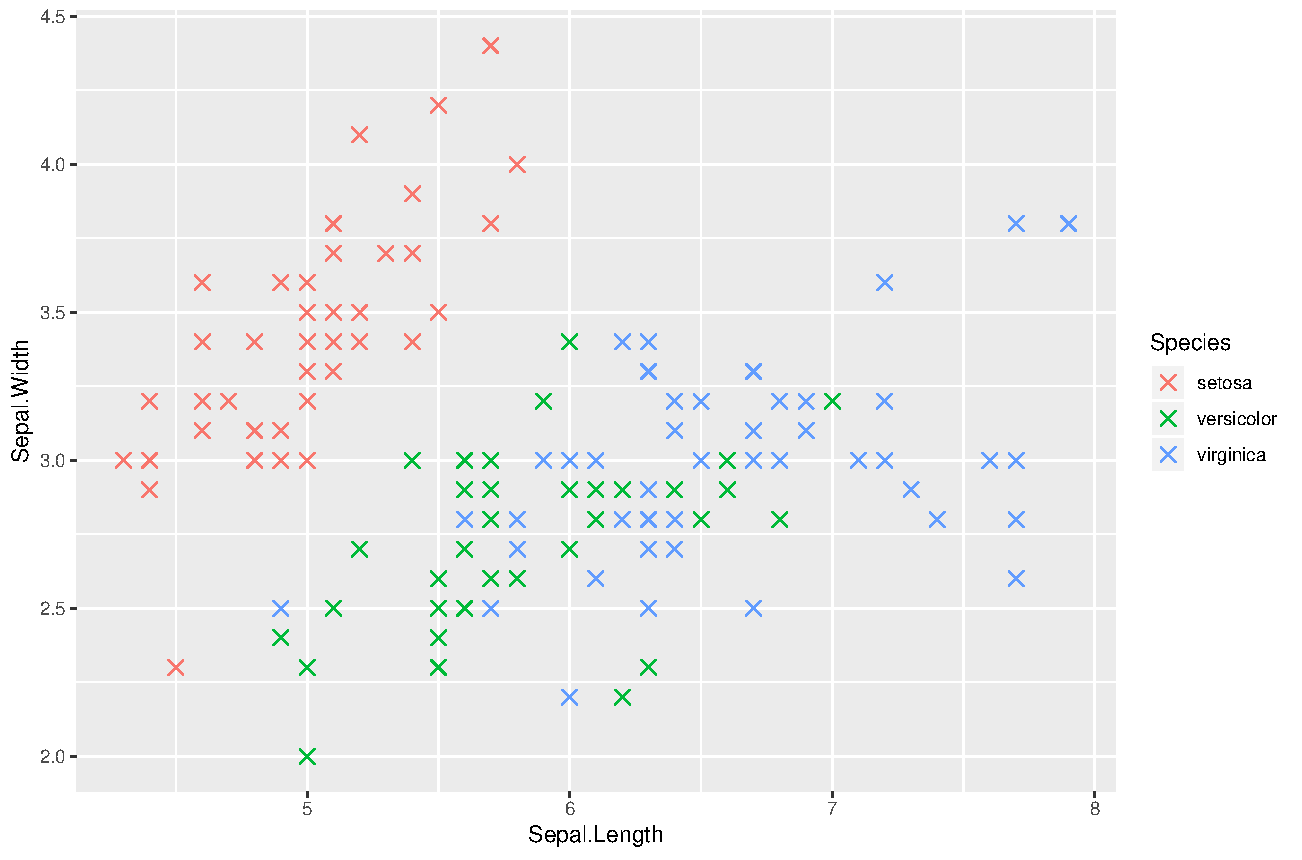
\includegraphics[scale=0.35]{pics/scatterggplot2.pdf}		
\end{figure} 
 
 
\end{itemize}




}
\end{frame}


\begin{frame}[fragile]{Scatter Plots (4)}
\scriptsize{
\begin{itemize}
 \item All pairs of the 4 variables of the iris dataset using a different color and character for each species:
 \begin{verbatim}
pairs(iris[,1:4],pch=as.numeric(iris$Species),col=iris$Species)
 \end{verbatim}

  \begin{figure}[h!]
	\centering
	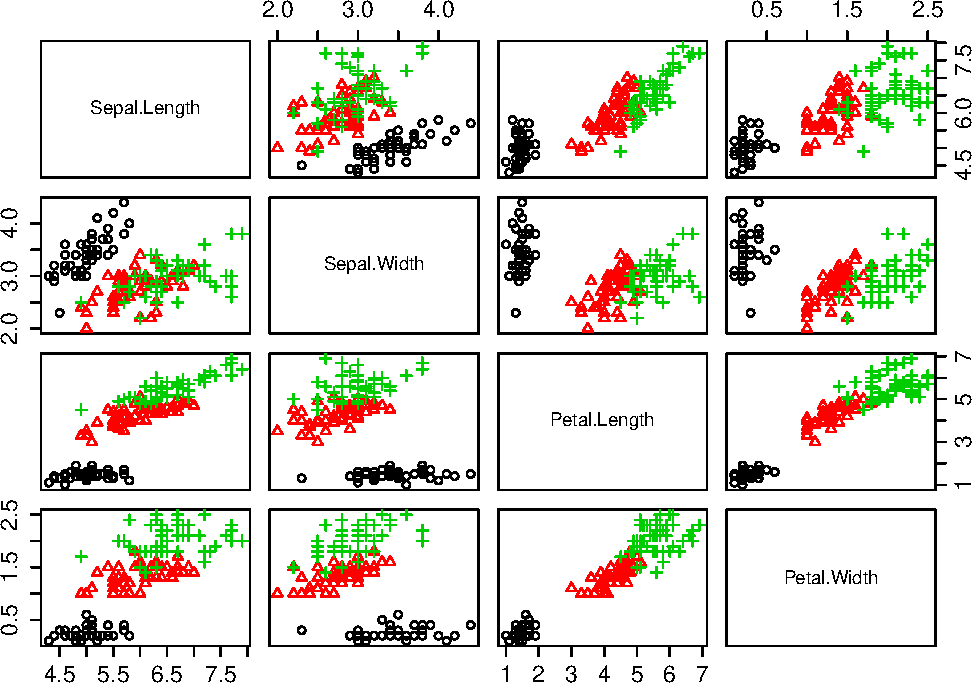
\includegraphics[scale=0.5]{pics/scatter2.pdf}		
\end{figure} 
 
 
\end{itemize}

}
 
\end{frame}


\begin{frame}[fragile]{Scatter Plots (5)}
\scriptsize{
\begin{itemize}
 \item Three-dimensional scatterplots can also be created.
 \item The \verb+scatterplot3d+ library must be installed using the following command:
 
 \begin{verbatim}
 install.packages("scatterplot3d",dependencies=T)
 \end{verbatim}
 
 \item Then load the library by typing \verb+library(scatterplot3d)+.
 
 \item A 3d scatterplot for petal width, sepal length and sepal width:
 \begin{verbatim}
scatterplot3d(iris$Petal.Width, iris$Sepal.Length, 
              iris$Sepal.Width, color=as.numeric(iris$Species),
              pch=as.numeric(iris$Species))  
 \end{verbatim}

 
  
\end{itemize}




}
 
\end{frame}


\begin{frame}[fragile]{Scatter Plots (6)}

 
 
  \begin{figure}[h!]
	\centering
	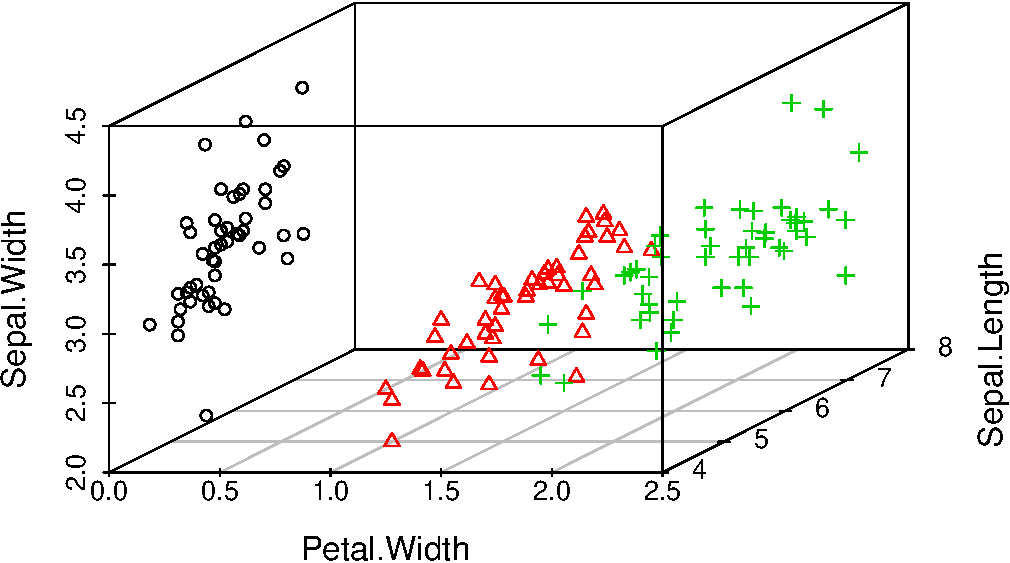
\includegraphics[scale=0.6]{pics/scatter3.pdf}		
\end{figure} 
 
 

 
\end{frame}



\begin{frame}[fragile]{Parallel Coordinate Plots}
\scriptsize{
 \begin{itemize}
  \item Parallel coordinate plots are another way to visualize multi-dimensional data.
  \item Instead of using perpendicular axes (x-y-z) we use several axes parallel to each other.
  \item Each attribute is represented by one of the parallel axes with its respective values.
  \item The values of the different attributes are scaled so that each axis has the same height.
  \item  Each observation represents a line that joins the different axes according to their values.
  \item In this way, examples similar to each other tend to be grouped in lines with similar trajectory.
  \item In many occasions it is necessary to re-order the axes in order to visualize a pattern.
 \end{itemize} 
 
 }  
\end{frame}


\begin{frame}[fragile]{Parallel Coordinate Plots (2)}
\scriptsize{
 \begin{itemize}
  \item  In R we can create parallel coordinate graphs with the command \verb+parcoord+ from the \verb+MASS+ library.
  \item Example:
  \begin{verbatim}
library(MASS)
parcoord(iris[1:4], col=iris$Species,var.label=T)   
  \end{verbatim}
  
  \begin{figure}[h!]
	\centering
	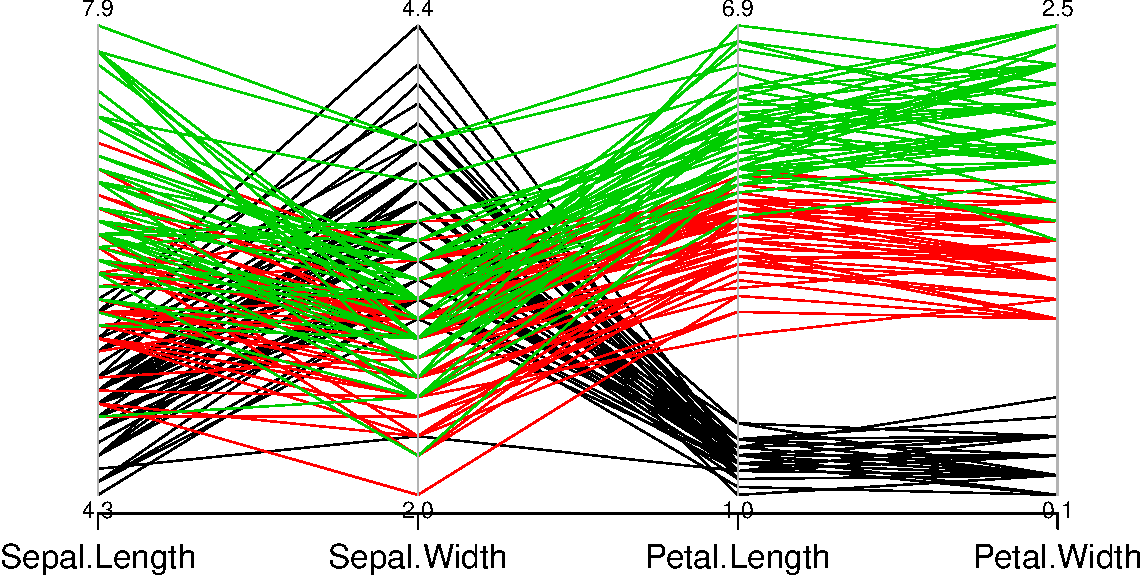
\includegraphics[scale=0.5]{pics/parallel.pdf}		
\end{figure}   

 \end{itemize} 
 
 }  
\end{frame}

\begin{frame}[fragile]{Conclusions}
\scriptsize{
 \begin{itemize}
  \item We have learned how to describe a dataset using various metrics and visualizations.
  \item These techniques give us a general understanding of the data.  
 \end{itemize} 
 
 }  
\end{frame}




%%%%%%%%%%%%%%%%%%%%%%%%%%%
%%%%%%%%%%%%%%%%%%%%%%%%%%%
\begin{frame}[allowframebreaks]\scriptsize
\frametitle{References}
\bibliography{bio}
\bibliographystyle{apalike}
%\bibliographystyle{flexbib}
\end{frame}  












%%%%%%%%%%%%%%%%%%%%%%%%%%%

\end{document}
